\cleartooddpage[\thispagestyle{empty}]
\chapter{Gamma Rays and Dark Matter}\label{ch_gamma}


This analysis searches for dark matter using gamma rays, thus a discussion on gamma rays and their properties is necessary.
The discussion revolves around three main topics: astrophysical mechanisms that create gamma rays, the production of gamma rays from the dark matter halo around the Galactic Center, and gamma-ray-induced air showers in the Earth's atmosphere.

\section{Methods of Creation}

  There are several mechanisms that can produce photons with TeV energies.
  A gamma ray can start as a thermal photon, then gain significant energy from interactions with electrons, referred to as a leptonic production.
  Alternately, a gamma ray can be created from a high-energy proton colliding with other matter, referred to as hadronic production.
  The primary mechanism this analysis searches for is the annihilation of two WIMP dark matter particles that either directly or indirectly produce gamma rays, and is discussed below.

  In leptonic production, electrons and low-energy photons collide, transferring energy to the photon.
  This interaction is called upscattering or Inverse Compton scattering~\cite{compton_effect}.
  While the chance that any one thermal photon will be upscattered to TeV energies is low, astrophysical scales involve large populations of photons and electrons.
  When these two populations interact, a small fraction of the original photon population can achieve TeV-scale energies~\cite{gammas_from_electrons}.

  In order to efficiently produce gamma rays via this method, a population of high-energy electrons is needed.
  One environment for producing these electrons is around pulsar wind nebulae.
  Due to their rapid rotation, pulsar wind nebulae are constantly twisting their magnetic field lines.
  These magnetic field lines occasionally break and reconnect, which temporarily create electric fields that can accelerate electrons outwards to higher energies than thermal sources (i.e. solar wind) alone can achieve~\cite{gamma_pwn1,gamma_pwn2}.

  Another mechanism that produces high-energy electrons is supernovae remnants.
  The supernova remnant consists of gas expanding into the surrounding interstellar gas, creating a moving shockfront at the boundary between these two volumes.
  Some charged particles in the expanding gas are able to cross the shockfront, where a small fraction will be reflected by magnetic fields.
  Upon recrossing the shockfront, they are again reflected by magnetic fields, which are expanding outwards with the supernova remnant gas, imparting energy to the charged particles.
  These particles repeatedly cross the shockfront, where a smaller and smaller fraction of particles gain more and more energy, in a mechanism called Fermi Acceleration~\cite{fermi1949,highenergyelectron_snr}.
  
  After either of these processes produce electrons with high energies, these electrons can then upscatter ambient photons to TeV energies.
  Additionally, electrons spiralling through magnetic fields can produce synchrotron photons at X-Ray energies, meaning fewer upscatters are needed to reach TeV energies~\cite{self_compton}.

  In hadronic processes, protons can be accelerated by fermi acceleraton or as part of an Active Galactic Nucleus jet~\cite{hadronic1,hadronic2}.
  Then, upon striking an ambient atom, the proton will {\color{red}convert (is convert the right word??)} into $\pi^{+}$, $\pi^{-}$, and $\pi^{0}$~\cite{pp_pion,pp_pion2}.
  The $\pi^{0}$ then quickly (\SI{8.5e-17}{s}~\cite{pdg2016}) decomposes into a $\gamma\gamma$ pair, with \nicetilde$10\%$ of the original proton's energy.
  Much of the diffuse gamma ray component of the galactic disk is due to extra-galactic high-energy protons colliding with the atoms of the dusty galactic plane~\cite{GalacticDiffuseGammaRays}.

  \subsection{Dark Matter Interactions}\label{dmgammaproduction}
    
    The dark matter particle searched for in this thesis is a WIMP, a particle predicted by SUSY.
    This WIMP may be detectable by three general search schemes, illustrated in Figure~\ref{fig:3_searches}.

    % add popular figure for the three detection type
    \begin{figure}[ht]
      \centering
      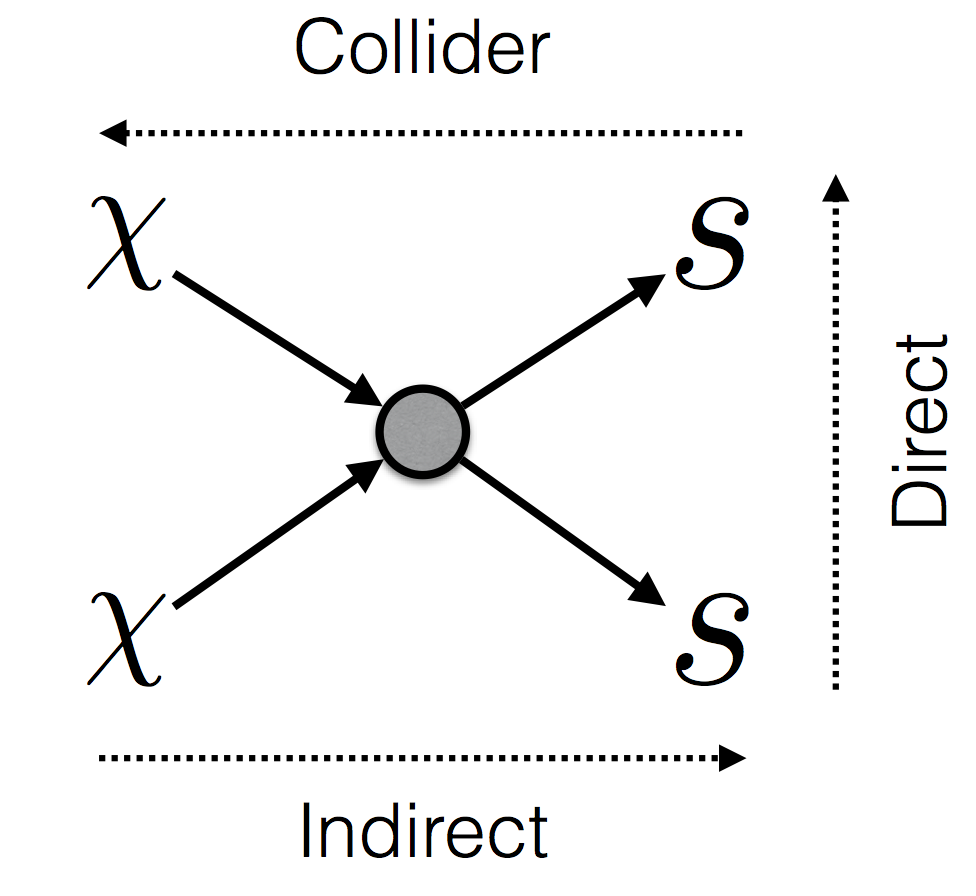
\includegraphics[width=0.65\textwidth]{images/3waystodetect/3waystodetect.pdf}
      \caption[3 Search Techniques]{
        The three general search techniques for dark matter.}
      \label{fig:3_searches}
    \end{figure}

    In Collider searches, $ss \rightarrow \chi\chi$, standard model particles ($ss$) are accelerated into each other within a detector, and the resulting particle fragments are measured by a slew of measuring equipment.
    {\color{red}Since the properties of the input accelerated particles are well known and the (?? this is not entirely true, the interior quarks and gluons can have different momentums, sentence should be more precise -Orel)} output fragment particles are well measured, searching for any break from {\color{red}conservation laws (?? The break from conservation laws does not yield dark matter particles. It can be used to search for them. Maybe ''suggest dark matter particles production``? --Orel)} may yield dark matter particles. {\color{red}(Sentence is fragmented, needs fixing)}
    {\color{red}This method has previously allowed for the discovery of many other new particles (?? Not accurate, most of these particles were detected directly through the particles they decayed to (like the higgs decaying to two photons). Dark matter would manifest as missing momentum since we cannot see the particles it decays to. -Orel)}, including the gluon in 1979~\cite{gluon_discovery}, the W and Z bosons in 1983~\cite{WZ_discovery1,WZ_discovery2}, the top quark in 1995~\cite{top_discovery}, the tau neutrino in 2000~\cite{tau_neutrino_discovery}, and the higgs boson in 2012~\cite{Higgs_ATLAS,Higgs_CMS}.

    For Direct searches, $\chi s \rightarrow \chi s$, sensitive particle detectors are built deep underground, where a dark matter particle impacting against an electron or nuclei creates a detectable recoil.
    This recoil can cause a detectable charge, an increase in temperature, an acoustic vibration, or a visual reaction like a photon or a gas bubble in a liquid, so detectors are built to measure some of these effects.
    However, to date no substantial dark matter signal has been detected with these methods~\cite{direct_dm_detection}.

    For Indirect searches, $\chi\chi \rightarrow ss$, astrophysical observations are analyzed for excess amounts of standard model particles, more than can be explained by known astrophysical processes.
    This analysis searches for an excess of gamma rays, as the center of our galaxy is believed to host a dark matter halo.
    This spherical halo would allow for many $\chi\chi$ annihilations, producing gamma rays via: 

    $$\chi\bar{\chi} \rightarrow S\bar{S} \rightarrow \gamma\gamma$$

    where $S\bar{S}$ can be any quark or lepton particle-antiparticle pair ($t\bar{t}$, $s\bar{s}$, $e^{-}e^{+}$, etc).
    These different annhilation channels can produce different spectra of gamma rays, which will also vary based on the WIMP mass and cross-section chosen.
    This is described further in Section \ref{dm_spectral}.

\FloatBarrier

\section{Galactic Center}

  The Galactic Center is a complex region of space, with many astrophysical sources of gamma rays.
  A disk of dust lies along the galactic plane, acting as an interaction medium for diffuse proton cosmic rays.
  Nearby supernova remnants also produce gamma rays as their expanding shells interact with ambient dust.
  The immediate area surrounding the Galactic Center contains a point-source gamma-ray emitter, although its mechanism is poorly understood.

  % black hole
  Through kinematic observations of nearby stars, it was deduced that the Galactic Center is home to a supermassive black hole, with a mass of \SI{4e6}{\Msol}~\cite{sgra_massdist}.
  The Galactic Center also is a source of \TeV{} gamma rays, though the mechanism that produces them is still under debate.
  One possibility is that the supermassive black hole accelerates protons to PeV energies, which then collide with local atoms to produce $\pi^0$s, which then decay into TeV gamma rays~\cite{gc_pevatron}.
  The second possibility suggests a nearby population of pulsar wind nebulae may be accelerating electrons, which then upscatter local photons to TeV energies~\cite{gc_pulsars}.
  While the Galactic Center is a source of gamma rays, the current generation of gamma-ray telescopes can only resolve it into a point source, due to their limited angular resolution~\cite{VeritasGCRidge2015,gc_pointsrc_hess}.

  The disk of gas present in the galactic plane acts as an interaction medium for passing cosmic rays, both from nearby galactic accelerators and from extragalactic sources.
  {\color{red}(discuss diffuse emission, can't find papers on it at TeV energies??)}

  {\color{red}(somewhere in thesis cite something from each defense committee member!)}

\section{Indirect Dark Matter Search}
  For this analysis, it is important to understand how a terrestrial telescope can detect the presence of dark matter.
  VERITAS can detect gamma rays that are emitted when two dark matter particles annihilate.
  Because the rate of annihilation depends on the local dark matter density, the radially-dependent structure of dark matter halos also affects the analysis.

  \subsection{Dark Matter and Gamma Rays}
    The main dark matter candidate searched for in this thesis is the WIMP particle.
    WIMPs are predicted to decay and self-annihilate into standard model particles.
    Primarily, indirect searches focus on annihilating WIMPs, as the predicted WIMP decay lifetime produces a lower flux of standard model particles than annihilation.
    WIMPs may annihilate into any standard model particle-antiparticle pair, but most studies examine a WIMP annihilating into a quark-antiquark pair, or a pair of gamma-ray photons.

    For example, two annihilating WIMPs may produce a $t\bar{t}$ pair, which then decays into... {\color{red}(?? The top decays to Wb 99.9\% of the time. -Orel)}.
    Or, they may produce $b\bar{b}$, or $\gamma\gamma$.

    These different annihilations will produce different spectra of final gamma rays.
  
  \subsection{Dark Matter Halo Structure}\label{dm_spatial}
    Observations allow most galactic dark matter halos to be modeled using a class of similar density profiles.
    A currently favored profile is the Einasto profile~\cite{einastoprofile1,einastoprofile2}.
    This profile describes the mass-density of dark matter at a distance r from the halo center, $\rho(r)$.
    The Einasto profile is described by Equation~\ref{eqn:einasto},

    \begin{equation} \label{eqn:einasto}
      \rho_{\textrm{DM}} \left( r \right) = \rho_{s} Exp \left( - \frac{2}{\alpha} \left( {\left( \frac{r}{r_s} \right)}^{\alpha} - 1 \right) \right)
    \end{equation}
    
    where $\alpha$ is fixed to 0.17, and $r_s$ is fixed to \SI{15.14}{kpc}.
    Both $\alpha$ and $r_s$ are from the best fit values of the Aq-A-1 simulation in Table 2 of Ref.~\cite{mw_halo_params}.
    The $r_s$ parameter is calculated via $r_s=r_{-2}=15.14\:\textrm{kpc}$, where $r_{-2}=\frac{11.05}{h}\:\textrm{kpc}$ (in Ref.~\ref{mw_halo_params}, Table 2) and $h=0.73$ from Section 2.1 in Ref.~\cite{mw_halo_params}.
    The distance to the galactic center is known to be $r_\odot=8\:\textrm{kpc}$~\cite{gc_distance_1,gc_distance_2,gc_distance_3}, and the local estimated dark matter mass density is $\rho_\odot = 0.4\:\frac{\textrm{GeV}}{\textrm{cm}^3}$~\cite{local_dm_density}, though this varies depending on the assumed Milky Way mass profile~\cite{direct_dm_astrophysical_uncertainties}.
    Since $r_\odot$ and $\rho_\odot$ are known, then in Equation~\ref{eqn:einasto} the dark matter density at the scale radius $\rho_s$ is derived to be \SI{0.12}{\GeV\per\cm^3}.
    With these values, the Einasto profile in Equation~\ref{eqn:einasto} is shown in Figure~\ref{fig:gchalo_density}.
  
    \begin{figure}[ht]
      \centering
      \includegraphics[width=0.95\textwidth]{images/halo/gc_einasto_profile.pdf}
      \caption[Galactic Center Einasto Halo Density]{
        Mass density of the Einasto dark matter halo used in this analysis.
        \CaptionBlankLine
        }
      \label{fig:gchalo_density}
    \end{figure}

    Other density profiles exist, but for this analysis only the Einasto profile is considered.
    Most simulations show that density profiles should terminate in a sharp peak at $r=0$, but observations of dwarf galaxies instead favor a flat core within a given radius~\cite{flores1994observational,CoreVsCusp}.
    This may be due to the presence of baryons in this core region, which can diffuse the central cusp of WIMPs into a core-like shape~\cite{corecusp_baryondiffuse1,corecusp_baryondiffuse2}.
    As this flat core occurs in the inner-most region covered by the gamma-ray observations in this analysis, the choice of a cuspy or cored dark matter halo can have a significant impact on this analysis.
    Specifically, if the dark matter halo follows a cored profile when using a cuspy halo model, then any derived upper limits on the dark matter cross-section would be different.
    For simplicity of implementation, only a cuspy halo is used in this thesis.
    
    When choosing which dark matter target to observe with a gamma-ray observatory, knowing the gamma-ray brightness of different sources can be useful.
    This Einasto density profile can be integrated to calculate this gamma-ray brightness, independent of the WIMP model being searched for.
    For annihilating dark matter, $\rho_{\textrm{DM}}\left(r\right)^2$ must be integrated along the line of sight.
    Equation~\ref{eqn:dmflux} can be used to calculate the amount of gamma rays produced by these annihilations.
    
    \begin{equation}\label{eqn:dmflux}
      \frac{ d\Phi }{ dE d \Omega } = \frac{ \left \langle \sigma v \right \rangle }{8 \pi m_\chi^2} \frac{dN_{\gamma}}{dE} \int \rho^2 dl
    \end{equation}
    
    In this equation, the photon flux $\Phi$ is the number of gamma rays detected per $\textrm{area}\times\textrm{time}$.
    The velocity-averaged cross-section of the dark matter candidate is $\left \langle \sigma v \right \rangle$.
    Velocity-averaging is used because the cross-section is velocity dependent, and the WIMPs that pass through a volume of space will have a distribution of velocities {\color{red}(cite??)}.
    Sometimes, part of Equation~\ref{eqn:dmflux} is calculated separately, as in Equation~\ref{eqn:jfactor}, and is referred to as the $J$ factor.

    \begin{equation}\label{eqn:jfactor}
      J = \int \rho^2 dl
    \end{equation}

    The $J$ factor is sometimes separately calculated to compare the relative gamma-ray brightness of different dark matter halos, which is a function of both dark matter density and observing distance.
    The Einasto density in Equation~\ref{eqn:einasto} can be integrated to calculate the $J$ factor at various radii, which is shown in Figure~\ref{fig:gchalo_jfactor}.
    The values in this figure are calculated using an integration radius of \ang{0.01}.
    The spectrum of photons produced by a single $\chi\chi$ annihilation is $\frac{dN_{\gamma}}{dE}$.
    
    \begin{figure}[ht]
    \centering
      \includegraphics[width=0.95\textwidth]{images/halo/gc_einasto_jfactor.pdf}
      \caption[Galactic Center Einasto Halo Jfactor]{
        J-factor profile as a function of angle from the Galactic Center.
        J-factor values are calculated with an integration angle of \ang{0.01}.
      }
      \label{fig:gchalo_jfactor}
    \end{figure}
    

    {\color{red}Sommerfield enhancement \url{https://arxiv.org/pdf/1005.4678.pdf} (??)}

    % from http://www.pnas.org/content/112/40/12264.full.pdf
    
    {\color{red}DM Flux skymap in galactic (l,b) ??}
    
    This J-factor profile then forms the spatial component of the dark matter halo, $M_{s,\textrm{halo}}$, used in Chapter~\ref{chapter:analysis}.
    
  \subsection{Spectrum of Gamma Rays from Dark Matter}\label{dm_spectral}
    In order to calculate the gamma-ray brightness of the dark matter halo, the produced spectrum from each WIMP annihilation must be known.
    Each WIMP annihilation can have distinct outcomes (each producing different pairs of particles), referred to as annihilation channels.
    WIMPs may annihilate directly into two gamma rays (the $\gamma\gamma$ channel), or may instead produce a quark-antiquark pair ($b\bar{b}$, $t\bar{t}$, ...), a lepton-antilepton pair, or almost any other standard model particle-antiparticle pair.

    Non-gamma-ray annihilation channels still indirectly produce gamma rays as the original particle pair decays.
    Many standard model particle-antiparticle annihilations also result in a mix of annihilation channels, so WIMPs may also have this feature.
    Mixing channels requires multiple dark matter halo models however, which is beyond the scope of this single halo analysis.
    The software package CLUMPY~\cite{CLUMPYcode} is used to calculate the gamma-ray spectra for each annihilation channel.
    The spectral models that CLUMPY uses are based on the tables in the PPPC 4 DM ID~\cite{pppc4_dm_spectra}.
    For this analysis, only the $b\bar{b}$ annihilation channel is considered.
    Figure~\ref{fig:chichi_spectrum} shows the resultant spectra from the single annihilation of two WIMPs.
    Each line shows the spectrum from a different initial WIMP mass.

    \begin{figure}[ht]
      \centering
      \includegraphics[width=0.95\textwidth]{images/spectra/chichi_spectrum.pdf}
      \caption[Single Annihilation Spectra]{
        Resultant photon spectra from a single annihilation of WIMP particles.
        Each colored line represents a different WIMP mass.}
      \label{fig:chichi_spectrum}
    \end{figure}

    These spectra are then stored in an interpolation table, which can be used as the spectral component $M_{\textrm{e,halo}}$ for the dark matter halo model in the likelihood analysis, detailed in Section~\ref{subsec:dmhalomodel}.
    These spectra can then be combined with J factor Equation~\ref{eqn:jfactor} to calculate Equation~\ref{eqn:dmflux}: how many gamma rays are produced by the halo.
    This is done in Equation~\ref{eqn:dmmodel}

    \FloatBarrier
    
    
\section{Atmospheric Showers}

  When a particle strikes an atom of Earth's atmosphere at GeV or higher energies, it can set off a cascade of energetic particles called an air shower~\cite{Bethe1934,Klein1999}.
  When the primary particle is composed of one or more baryons, like a proton or Iron atom, it creates a hadronic shower.
  When the primary is a gamma ray or a charged lepton, it creates an electromagnetic shower.
  Electromagnetic showers produce a cascade of $e^{\pm}$s and $\gamma$'s, where each successive generation of particles tends to have more particles but less energy per particle than the last.
  To start the shower, the primary gamma ray will interact with an atmospheric atom, producing an $e^{-}e^{+}$ pair, each with roughly half the primary gamma ray's energy, as shown in Figure~\ref{fig:emcascade}.
  The $e^{-}$ and $e^{+}$ may emit some photons as bremstrahlung radiation, and then {\color{red}collide with other atmospheric atoms to produce more $e^{-}e^{+}$ pairs (?? The photons are the ones which produce more e+e- pairs -Orel)}.
  As each newly created particle has less energy than its parent particle, eventually the particles in the shower don't have enough energy to produce additional child-particles.
  This occurs when electrons have around \SI{80}{MeV} of kinetic energy, where they rapidly lose energy to ionization~\cite{pdg_2014}.

  %\begin{figure}[ht]
  %  \centering
  %  \includegraphics[width=0.85\textwidth]{images/cascade_diagram/emcascadegv.pdf}
  %  \caption[Electromagnetic Cascade]{
  %    Diagram of an electromagnetic cascade as it decends downwards through the atmosphere, layered by interaction generation.
  %    $\gamma{}o$ is the initial astrophysical gamma ray, and continues for many generations after these first four.
  %    {\color{red}(?? Only gamma's should pair produce, leptons should only bremstrahlung, since leptons only pair-convert when they're below the 80MeV.)}
  %    {\color{red}(?? Photons are bosons, in feynman diagrams should have wiggly lines!)}
  %  }
  %  \label{fig:emcascade}
  %\end{figure}

  \begin{figure}[ht]
    \centering
    \includegraphics[width=0.95\textwidth]{images/cascade_diagram/feynman/cascade.pdf}
    \caption[Electromagnetic Cascade]{
      Diagram of an electromagnetic cascade as it decends downwards through the atmosphere, layered by interaction generation.
      $\gamma{}_o$ is the initial astrophysical gamma ray.
      The shower shown here continues for many generations after these first four.
      Diagram produced with the TikZ-Feynman package~\cite{ellis2017tikz}.
    }
    \label{fig:emcascade}
  \end{figure}

  (\nicetilde 99\%) of detected air showers are due to {\color{red}protons and not gamma rays (what about electron showers??)}.
  Understanding the differences between hadronic and electromagnetic showers is useful for removing unwanted proton events and preserving gamma-ray events within the reconstruction method, sometimes referred to as gamma-hadron separation.
  Hadronic showers start with a primary \nicetilde TeV proton that interacts with an atmospheric atom.
  {\color{red}This proton then converts (?? It doesn't convert to pions. Definately not to pi+ pi- adn pi0, (charge conservation). -Orel)} into $\pi^{+}$, $\pi^{-}$, and $\pi^{0}$, each with roughly \nicetilde $\frac{1}{3}$ of the initial proton's energy.
  {\color{red}(Include feynman diagrams of proton->pion and pion->gammagamma ?? )}
  {\color{red}(?? Isn't there also a neutron in some diagrams??)}
  % see here for neutron: https://en.wikipedia.org/wiki/Cosmic_ray
  The $\pi^{+}$ and $\pi^{-}$ can travel far in the tranverse direction, away from the main axis of the primary particle, then decay into $\mu^{+}\nu_{\mu}$ and $\mu^{-}\bar{\nu}_{\mu}$ pairs, respectively.
  The $\pi^{0}$ quickly decays into pair of gamma rays, each of which then start their own electromagnetic shower.
  The $\pi^{+}$ and $\pi^{-}$ have longer decay times ($\pi^{\pm} \rightarrow $\SI{3e-8}{s} vs $\pi^{0} \rightarrow $\SI{9e-17}{s}~\cite{pdg_2014}), allowing them to carry energy farther away from the central shower axis.
  Both of these effects create sub-showers farther away from the primary particle axis, which tends to cause hadronic showers (and their resulting Cherenkov images, discussed in Section \ref{sec:cherenkov}) to be wider than a purely electromagnetic shower of the same length. 
  
  In Figure~\ref{fig:gamma_vs_proton_airshower}, the differences between a gamma-ray shower and a proton shower are shown.
  The gamma-ray shower on the left has most of its particles along the veritical core of the shower, while the proton shower has particles spread out in a wider, fan-like shape.
  The initial energies were chosen because a \SI{1}{TeV} proton will on average divest $\frac{1}{3}$ of its energy to the $\pi^{0}$.

  This $\pi^{0}$ then decays into the electromagnetic sub-shower faintly visible in the interior of the proton shower.
  The net effect is that, when compared to a gamma ray, a proton must start with 3 times the energy to produce a similar amount of Cherenkov photons, which are distributed in a wider pattern.

  \begin{figure}[ht]
    \centering
    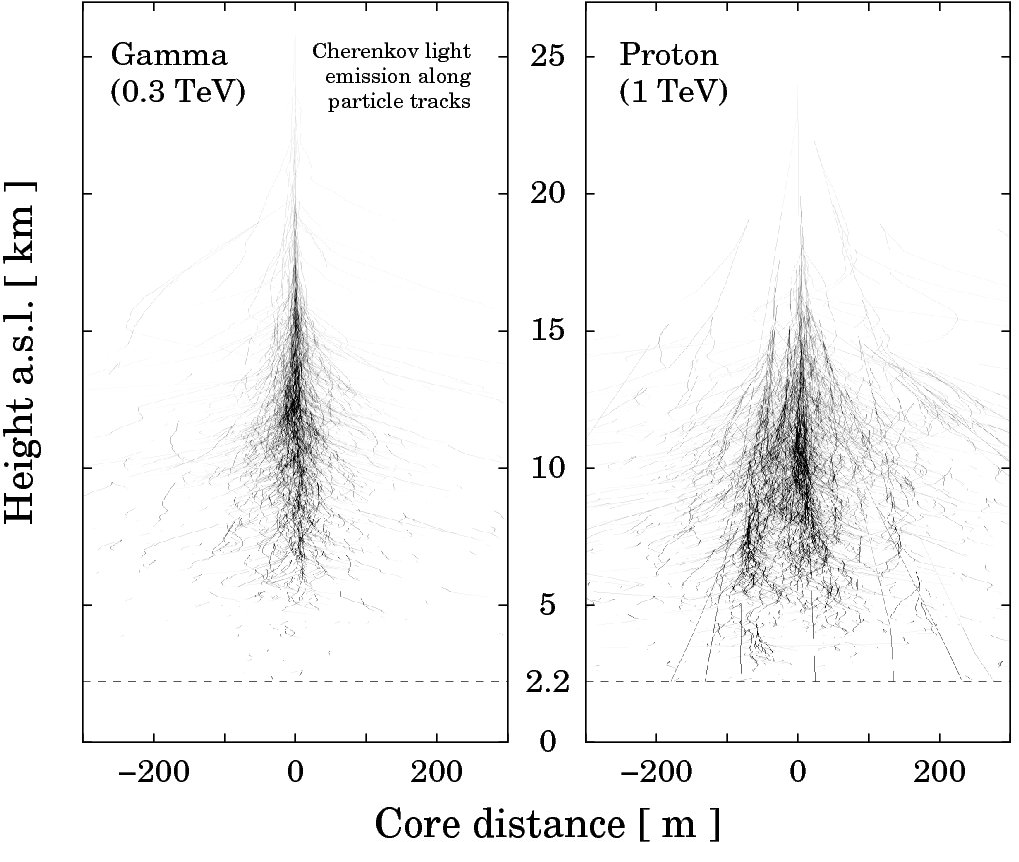
\includegraphics[width=0.95\textwidth]{images/showers_gamma_proton}
    \caption[Gamma Ray and Proton Showers]{
      A gamma ray shower alongside a proton shower~\cite{Bernlohr2008149}.
    }
    \label{fig:gamma_vs_proton_airshower}
  \end{figure}
  
  \FloatBarrier

  \subsection{Cherenkov Photons}\label{sec:cherenkov}

  Within atmospheric showers, any charged particles travelling at velocity $v > c_{atmosphere}$ will induce the atmosphere to produce Cherenkov photons~\cite{cherenkov}, where $c$ is the speed of light in the atmosphere.
  From a single charged particle of constant velocity, Cherenkov photons form a conical wavefront shown in Figure~\ref{fig:cherenkovangle}, similar to a sonic boom shockwave or the wake produced when a boat travels faster than the speed of the waves.

  \begin{figure}[ht]
    \centering
    \includegraphics[width=0.27\textwidth]{images/cherenkov_angle/cherenkovangle.pdf}
    \caption[Chernekov Emission Angle]{
      Cherenkov light (blue arrows) is emitted at angle $\theta$, relative to the charged particle z's path.
    }
    \label{fig:cherenkovangle}
  \end{figure}

  Cherenkov photons are produced at an angle $\theta$ relative to the charged particle's path, determined by the index of refraction of the medium $n$, the speed of the charged particle $v$, and the speed of light in the medium $c$, as in Equation~\ref{eqn:cherenkovangle}.

  \begin{equation}\label{eqn:cherenkovangle}
    \theta = ArcCos \left ( \frac{c}{n \; v} \right )
  \end{equation}
  
  For the gamma-ray showers used in this analysis, the cherenkov angle $\theta$ is \nicetilde\ang{1}.
  % showers are 10km up, light pool on ground is 130m diameter, \theta = ArcSin(130/10000) * 180 / pi = 0.73deg ~ 1deg

  However in an atmospheric shower, the number and distribution of charged particles and their velocities, as well as energy losses, tend to smear the theoretically-clean Cherenkov cones into a diffuse pool of light on the ground, shown in Figure~\ref{fig:lightpool}.

  \begin{figure}[ht]
    \centering
    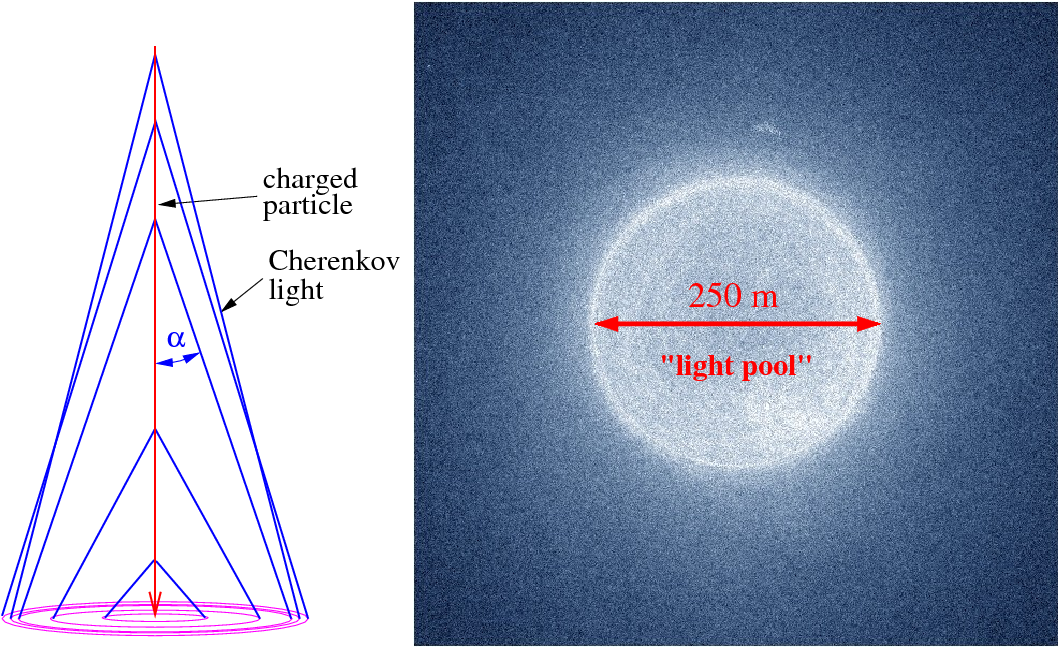
\includegraphics[width=0.85\textwidth]{images/lightpool/lightpool.pdf}
    \caption[Chernekov Light Pool]{
      Cherenkov light from a gamma ray shower illuminating the ground.
      Due to the changing atmospheric density, the cherenkov angle changes as the electromagnetic shower decends (Left), concentrating the emitted light into a ring-like pool (Right).
      The initial gamma ray had an energy of \SI{1}{\TeV}.
      Figure is from Ref.~\cite{Voelk}.
    }
    \label{fig:lightpool}
  \end{figure}
  
  The spectrum of photons produced by the Cherenkov effect can be calculated with the Frank-Tamm formula~\cite{franktamm1,franktamm2} in Equation~\ref{eqn:franktamm},
  
  \begin{equation}\label{eqn:franktamm}
    \frac{dE}{dx\,d\omega}=\frac{(ze)^2 \, \omega}{c^2} \left ( 1 - \frac{c^2}{v^2 \;\epsilon(\omega)} \right )
  \end{equation}
  
  where $E$ is the energy emitted as Cherenkov radiation, $x$ is the length of the charged particle path, $ze$ is the charge of the particle, $\omega$ is the emitted Cherenkov photon frequency, $c$ is the speed of light (phase velocity) in the medium, $v$ is the speed of the particle, and $\epsilon(\omega)$ is the frequency-dependent permittivity.
  The UV- and Visible-spectrum Cherenkov photons are then imaged and recorded by the VERITAS observatory.
  {\color{red}(Why just those frequencies?? does the cerenkov spectrum cutoff, or atmospheric absorption??)}
  {\color{red}(?? I think UV is absorbed by the atmosphere almost completely no?  Either way, those are the frequencies imaged because they are the ones Cherenkov light -Orel)}
  
  \begin{figure}[ht]
    \centering
    \includegraphics[width=0.75\textwidth]{images/CherenkovReactor/cherenkovreactor.eps}
    \caption[Chernekov Light from a Reactor]{
      Blue Cherenkov light in the Advanced Test Rector core, at the Idaho National Laboratory~\cite{cherenkovreactor,atrlab}.
    }
    \label{fig:cherenkovreactor}
  \end{figure}
  
  In Figure~\ref{fig:cherenkovreactor}, a visible example of Cherenkov photons is shown, produced in the Advanced Test Reactor at the Idaho National Laboratory.
  Neutrons emitted by the reactor collide with atoms in the water, freeing some electrons with enough kinetic energy to travel faster than the speed of light in water.
  These superluminal-in-water electrons then create the blue Cherenkov photons imaged here.
  
